% Kompilieren mit: TEXINPUTS=minted/source: xelatex -shell-escape %
\documentclass[12pt,compress,ngerman,utf8,t]{beamer}
\usepackage[ngerman]{babel}
\usepackage{comment}
\usepackage{minted}
\setminted{linenos}
\usepackage[protrusion=true,expansion=false]{microtype}

\DeclareSymbolFont{extraup}{U}{zavm}{m}{n}
\DeclareMathSymbol{\varheart}{\mathalpha}{extraup}{86}
\DeclareMathSymbol{\vardiamond}{\mathalpha}{extraup}{87}

\title{Monadische Parserkombinatoren}
\author[Curry Club Augsburg]{\texorpdfstring{
  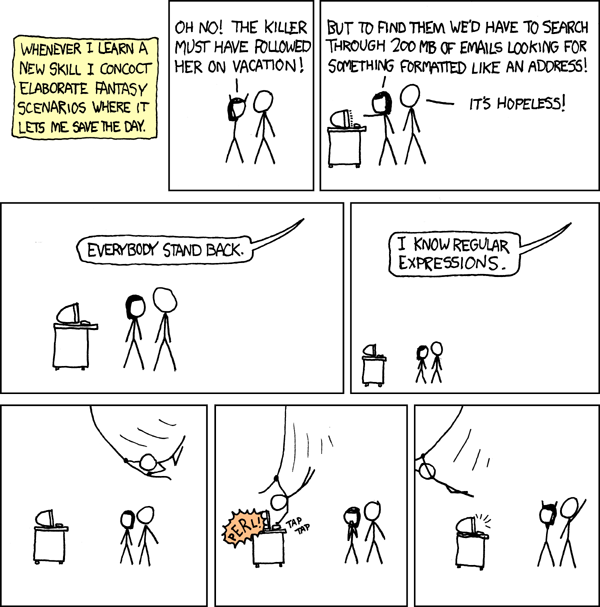
\includegraphics[scale=0.26]{images/regex} \\[0.7em]
  \scriptsize Ingo Blechschmidt \\\texttt{<iblech@speicherleck.de>}
}{Ingo Blechschmidt}}
\date{23. April 2015}

\usetheme{Warsaw}

\useinnertheme{rectangles}

\usecolortheme{seahorse}
\definecolor{mypurple}{RGB}{150,0,255}
\setbeamercolor{structure}{fg=mypurple}

\usefonttheme{serif}
\usepackage{fontspec}
\defaultfontfeatures{Mapping=tex-text}
\setmainfont{Linux Libertine O}

\setbeamertemplate{navigation symbols}{}
\setbeamertemplate{headline}{}

\setbeamertemplate{title page}[default][colsep=-1bp,rounded=false,shadow=false]
\setbeamertemplate{frametitle}[default][colsep=-2bp,rounded=false,shadow=false,center]

\newcommand*\oldmacro{}%
\let\oldmacro\insertshorttitle%
\renewcommand*\insertshorttitle{%
  \oldmacro\hfill\insertframenumber\,/\,\inserttotalframenumber\hfill}

\newcommand{\hil}[1]{{\usebeamercolor[fg]{item}{\textbf{#1}}}}

\begin{document}

\frame{\titlepage}

\begin{frame}[fragile]\frametitle{Ziel: S-Ausdr"ucke parsen}
  \begin{minted}{haskell}
data Exp = Atom String | List [Exp]

-- Eingabe:
(+ 1 (* 2 3) (* 4 5))

-- Syntaxbaum:
List
    [ Atom "+"
    , Atom "1"
    , List [ Atom "*", Atom "2", Atom "3" ]
    , List [ Atom "*", Atom "4", Atom "5" ]
    ]
  \end{minted}
\end{frame}

\begin{frame}[fragile]\frametitle{Ziel: S-Ausdr"ucke parsen}
  \begin{minted}{haskell}
data Exp = Atom String | List [Exp]

parseExp :: Parser Exp
parseExp = choice [ parseSymbol, parseList ]

parseSymbol :: Parser Exp
parseSymbol =
    fmap Atom $ many1 alphaNum `andThen` spaces

parseList :: Parser Exp
parseList = do
    token "("
    elems <- many parseExp
    token ")"
    return $ List elems
  \end{minted}
\end{frame}

\begin{frame}
  \begin{center}
    % http://learnyouahaskell.com/introduction
    
\includegraphics[scale=0.5]{images/bird}

    \huge
    Live-Coding
    \bigskip

    \large
    \texttt{\$ vim parsen-macht-spa"s.hs}
  \end{center}
\end{frame}

\begin{frame}\frametitle{Was fehlt noch?}
  \begin{itemize}
    \item Unsere naive Bibliothek leckt Speicher.
    \item Wir geben keine guten Parse-Fehlermeldungen aus.
    \item Wir haben keine Kombinatoren zum Parsen von Termen mit Operatoren.
  \end{itemize}
\end{frame}

\begin{frame}
  \begin{center}
    
\includegraphics[scale=0.4]{images/monadic-parser-combinators.jpeg}
  \end{center}
\end{frame}

\end{document}
